\documentclass[portrait,a1,final]{a0poster}

\usepackage{ssgposter}
\usepackage[utf8]{inputenc}
\usepackage[english]{babel}
\usepackage[SCI,RGB]{aaltologo}
\usepackage{lipsum}
\usepackage{graphicx}
\usepackage{float}

\begin{document}

\title{Zero Trust Architecture on K8s sidecars}
\author{Aarni Halinen, José Luis Martin Navarro, Jacopo Bufalino}

\makeheader

\begin{minipage}{\posterwidth}
  % Single column
  \begin{minipage}{\singlecolumnwidth}
    \section*{\sectiontitle{Problem}}
    \begin{itemize}
      \item Kubernetes applications often use co-scheduled sidecar containers for peripheral tasks like logging, observability...
      \item Sidecar containers reside in same Pod with the main container for co-scheduling, and communicate via loopback device
      \item Network policies can only be applied to Pod-to-Pod communication
      \begin{itemize}
        \item Sidecar receives same network access rules as the main application container
        \item No built-in tooling for filtering traffic between the main container and the sidecar
      \end{itemize}
      \item Egress traffic from the sidecar is indistinguishable from the main container
    \end{itemize}
  \end{minipage}

  % Left column
  \begin{minipage}[t]{\doublecolumnwidth}
    \vspace{\sectionspace}
    \section*{\sectiontitle{Solution 1}}

    On Linux systems,


    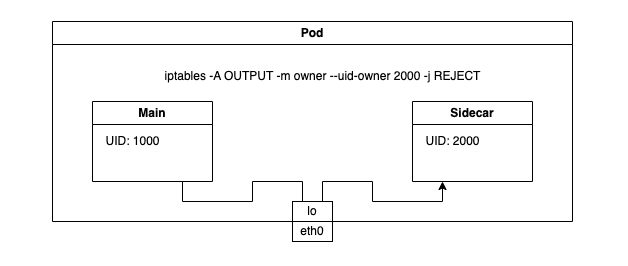
\includegraphics[width=\linewidth]{figures/iptables.png}
  \end{minipage}
  \hspace{\columnspace}
  % Right column
  \begin{minipage}[t]{\doublecolumnwidth}
    \vspace{\sectionspace}
    \section*{\sectiontitle{Solution 2}}

    Another approach With \emphasis{macvlan} CNI and \emphasis{Multus}, a CNI plugin that allows creation of multiple network interfaces per Pod, a new bridge network can be created between the Pods. This network has own IP address space, and is independent from Network Policies applied on the default cluster network. For forwarding all \emphasis{localhost} traffic to the new network, a DNAT routing rule can be attached to the loopback devices. The functionality of Network Policies can be implemented on the bridge network with \emphasis{MultiNetworkPolicy}, a custom resource definition provided by the same team behind the Multus CNI.

    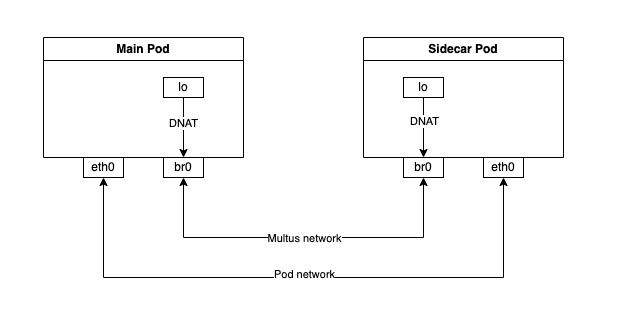
\includegraphics[width=\linewidth]{figures/multus.png}
  \end{minipage}
\end{minipage}

\section*{\sectiontitle{Colors}}
\begin{itemize}
        \item Use \emphasis{blue} for emphasis
        \item Use \negative{red} for negative points
        \item Use \positive{green} for positive points
\end{itemize}

\makefooter
  {
    aarni.halinen@aalto.fi,
    jose.martinnavarro@aalto.fi,
    jacopo.bufalino@aalto.fi
  }
\end{document}
